\documentclass[a4paper,12pt]{report}

%Русский язык
\usepackage[T2A]{fontenc}
\usepackage[utf8]{inputenc}
\usepackage[english,russian]{babel}
\usepackage{cmap}

%Работа с кодом
\usepackage{listings}
\usepackage{color}

\definecolor{green}{rgb}{0,0.6,0}
\definecolor{gray}{rgb}{0.5,0.5,0.5}
\definecolor{red}{rgb}{0.6,0,0}

\lstset{
        language=Python, 
        basicstyle=\small\ttfamily, 
        numberstyle=\tiny,           
        columns=flexible,
        stepnumber=1,                   
        numbersep=5pt,        
        showspaces=false,
        showstringspaces=false,
        showtabs=false,
        tabsize=2,                
        captionpos=b,              
        breaklines=true,           
        breakatwhitespace=false,
        keywordstyle=\color{green},
        commentstyle=\color{gray},
        stringstyle=\color{red},      
}

%Математика
\usepackage{amsmath,amsfonts,amssymb,amsthm,mathtools}
\usepackage{gensymb} 

%Изображения
\usepackage{float}
\usepackage{graphicx}
\graphicspath{ {./img/} }

%Поля страницы
\usepackage{geometry} 
\geometry{left=2.3cm} 
\geometry{right=1.8cm} 
\geometry{top=2cm} 
\geometry{bottom=2.5cm} 

%Отступы
\usepackage{indentfirst}
\setlength{\parskip}{0cm}

%Источники
\addto\captionsrussian{\def\refname{Список использованных источников}}

\begin{document} 

\begin{titlepage}
\newpage
	\begin{center}
		\large Санкт-Петербургский политехнический университет Петра Великого\\
		Институт компьютерных наук и технологий\\
		Высшая школа интеллектуальных систем и суперкомпьютерных технологий\\
	\end{center}
\vspace{7cm}

\begin{center}
		\large \textbf{Отчёт по лабораторной работе №2} \\
		\textbf{Дисциплина:} Телекоммуникационные технологии\\
		\textbf{Тема:} Гармоники
\end{center}
\vspace{4cm}
	
\begin{flushright}
		\large Работу выполнил:\\ Ляшенко В.В.\\
		Группа: 3530901/80201\\
		Преподаватель:\\ Богач Н.В.
\end{flushright}

\vspace{\fill}
\begin{center}
	\large Санкт-Петербург\\ 2021
	\end{center}
\end{titlepage}

\tableofcontents
\listoffigures
\lstlistoflistings

\chapter{Свойства преобразования Фурье}
\section{Преобразование Фурье}
    Преобразование Фурье – интегральное преобразование, которое является инструментом спектрального анализа непериодических сигналов. Для периодических сигналов используется дискретное преобразование Фурье.
    
    Прямым преобразованием Фурье функции $f(t)$ называется следующая функция (при условии, что интеграл сходится):
\begin{equation}
       F(\omega) = \int_{-\infty}^{\infty} f(t) e^{-j \omega t} dt
\end{equation}
    
    Обратное преобразование в этом случае задается формулой:
\begin{equation}
       f(t) = \frac{1}{2\pi} \int_{-\infty}^{\infty} F(\omega) e^{j \omega t} d \omega
\end{equation}

\section{Свойства}
\subsection{Линейность}
    Преобразование Фурье относится к числу линейных интегральных операций, т.е. спектр суммы сигналов равен сумме спектров этих сигналов.
\begin{equation}
       \sum \limits_{i} a_i f_i(t) \Leftrightarrow \sum \limits_{i} a_i F_i(\omega)
\end{equation}  

\subsection{Смещение}
    При смещении функции по аргументу на $t_0$ её ПФ умножается на $e^{j \omega t}$.
 \begin{equation}
       F(\omega) = \int_{-\infty}^{\infty} f(t+t_0) e^{-j \omega t} dt =  \int_{-\infty}^{\infty} f(t+t_0) e^{-j \omega (t+t_0)} d(t+t_0) e^{-j \omega (-t_0)} = e^{j \omega t_0} S(\omega)
\end{equation}    

\subsection{Изменение масштаба}
    Если аргумент $t$ функции $f(t)$ заменить на $at$, где $a$ постоянный коэффициент, то ПФ функции с $F(\omega)$ изменится на $\frac{1}{|a|}F(\frac{\omega}{a})$.
\begin{equation}
       F(\omega) = \int_{-\infty}^{\infty} f(at) e^{-j \omega t} dt = \frac{1}{a}\int_{-\infty}^{\infty} f(at) e^{-j \frac{\omega}{a} at} d(at)=\frac{1}{|a|}F(\frac{\omega}{a})
\end{equation}

    Появление модуля коэффициента $a$ вызвано тем, что при отрицательном значении коэффициента замена переменной приводит к изменению  знаков у пределов интегрирования.

    Из равенства следует, что сжатие функции $f(t)$ по времени в $a$ приводит к расширению по частоте в $a$ соответствующего ПФ и наоборот -  расширение функции приводит к сжатию ПФ.  
    
\subsection{Дифференцирование}
    При дифференцировании функции $f(t)$ её ПФ умножается на $j\omega$.
    
    Для доказательства используем определение понятия производной:
\begin{equation}
       f(t) = \frac{df}{dt} = \lim \frac{f(t+\varepsilon)-f(t)}{\varepsilon}
\end{equation}    

    Применим к этому выражению ПФ:
\begin{equation}
       F(\omega) = \int_{-\infty}^{\infty} \lim_{\varepsilon\to\\0} \frac{f(t+\varepsilon)-f(t)}{\varepsilon} e^{-j \omega t} dt = \lim_{\varepsilon\to\\0} \frac{S(\omega)e^{j \omega \varepsilon} - S(\omega)}{\varepsilon} = S(\omega)\lim_{\varepsilon\to\\0} \frac{e^{j \omega \varepsilon} - 1}{\varepsilon} = j \omega S(\omega)
\end{equation} 

    При дифференцировании низкие частоты ослабляются, а высокие усиливаются. Фазовый спектр сигнала сдвигается на 90\degree для положительны частот и на -90\degree для отрицательных.    
     
\subsection{Интегрирование}
    Интегрирование является операцией обратной дифференцированию. Логично предположить, что при интегрировании функции $f(t)$ её ПФ делится на $j\omega$. Но это утверждение справедливо только для сигналов, не имеющих постоянной составляющей.
\begin{equation}
       S(0) = \int_{-\infty}^{\infty} f(t) dt = 0
\end{equation}     

    В общем случае результат должен содержать дополнительное слагаемое в виде дельта-функции на нулевой частоте.
\begin{equation}
       F(\omega) = \frac{S(\omega)}{j\omega}+\pi S(0) \delta(\omega)
\end{equation}

    При интегрировании исходного сигнала высокие частоты ослабляются, а низкие усиливаются. Фазовый спектр сигнала сдвигается на -90\degree для положительны частот и на 90\degree для отрицательных. 
\subsection{Свертывание}
    ПФ свертки двух функций равно произведению ПФ свертываемых функций.
\begin{equation}
       f(t) = \int_{-\infty}^{\infty} s(f')g(t-t') dt'
\end{equation}

    Подвергнем такую конструкцию ПФ.
\begin{equation}
       F(\omega) = \int_{-\infty}^{\infty} \int_{-\infty}^{\infty} s(f')g(t-t') dt' e^{-j \omega t} dt = \int_{-\infty}^{\infty} s(f') e^{-j \omega t'} \int_{-\infty}^{\infty} g(t-t') e^{-j \omega (t-t')}d(t-t')dt' = S(\omega)G(\omega)
\end{equation}
    
\subsection{Произведение}
    Спектр произведения является сверткой спектров. Докажем это.
\begin{equation}
       f(t) = s(t)g(t)
\end{equation}    
    
    Тогда:
\begin{eqnarray}
       F(\omega) = \int_{-\infty}^{\infty} s(t)g(t) e^{-j \omega t} dt = \int_{-\infty}^{\infty} \Bigg( \frac{1}{2\pi} \int_{-\infty}^{\infty} S(\omega ') e^{j \omega ' t} d \omega ' \Bigg)g(t)e^{-j \omega t} dt =\nonumber\\
        = \frac{1}{2\pi} \int_{-\infty}^{\infty} S(\omega ') \int_{-\infty}^{\infty} g(t) e^{-j (\omega-\omega ') t} dt d \omega ' = \frac{1}{2\pi} \int_{-\infty}^{\infty} S(\omega ')G(\omega - \omega ') d\omega '
\end{eqnarray}    

\chapter{Упражнение 2.1}
    В начале мы должны для Jupyter загрузить \texttt{chap02.ipynb}, прочитать пояснения и запустить примеры.
    
    Все примеры были успешно запущены. В последнем примере при низких значений \texttt{freq} звук похож на гудение, а при высоких - на скрежет. При изменениях параметра \texttt{framerate} звук получался более приглушённым или наоборот более слышимым (Рис.2.1).
\begin{figure}[H]
        \centering
        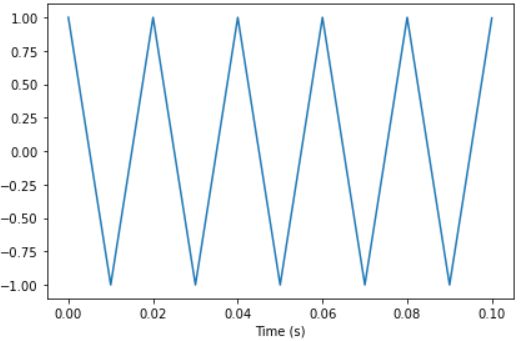
\includegraphics[width=0.8\textwidth]{fig2-1.PNG}
        \caption{Использование интерактивных виджетов IPython}
        \label{fig:fig2-1}
\end{figure}

\chapter{Упражнение 2.2}
\section{Пилообразный сигнал}
    Напишем класс \texttt{SawtoothSignal}, расширяющий \texttt{Sinusoid} и предоставляющий \texttt{evaluate} для оценки пилообразного сигнала.
    
\begin{lstlisting}[caption=Класс пилообразного сигнала]
from thinkdsp import Sinusoid, normalize, unbias, PI2
import numpy as np
class SawtoothSignal(Sinusoid):

    def evaluate(self, ts):
        cycles = self.freq * ts + self.offset / PI2
        frac, _ = np.modf(cycles)
        ys = normalize(unbias(frac), self.amp)
        return ys
\end{lstlisting} 
    
    Проверим, что сигнал генерируется правильно (Рис.3.1).
\begin{lstlisting}[caption=Генерация пилообразного сигнала]
    signal = SawtoothSignal()
    sawtooth_wave = signal.make_wave(signal.period*5, framerate=10000)
    sawtooth_wave.plot()
    decorate(xlabel='Time (s)')
\end{lstlisting}  

\begin{figure}[H]
        \centering
        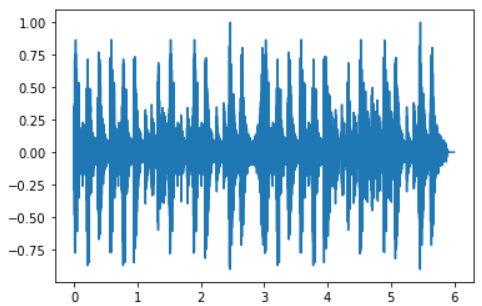
\includegraphics[width=0.8\textwidth]{fig3-1.PNG}
        \caption{Пилообразный сигнал}
        \label{fig:fig3-1}
\end{figure}    

\section{Спектр пилообразного сигнала} 
    Теперь вычислим спектр пилообразного сигнала (Рис.3.2).  
\begin{lstlisting}[caption=Вычисление спектра пилообразного сигнала]
    sawtooth_wave = signal.make_wave(duration=0.5, framerate=40000)
    sawtooth_wave.apodize()
    spectrum = sawtooth_wave.make_spectrum()
    spectrum.plot()
    decorate(xlabel='Frequency (Hz)')
\end{lstlisting}

\begin{figure}[H]
        \centering
        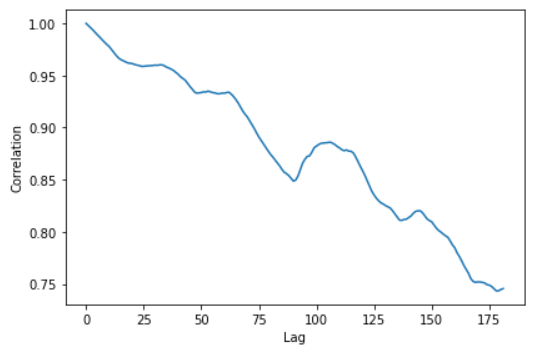
\includegraphics[width=0.8\textwidth]{fig3-2.PNG}
        \caption{Спектр пилообразного сигнала}
        \label{fig:fig3-2}
\end{figure} 

    Сравним гармоническую структуру пилообразного сигнала с треугольным и прямоугольным сигналами.
    
    Сначала сравним с треугольным сигналом.
\begin{lstlisting}[caption=Сравнение с треугольным сигналосм]
    from thinkdsp import TriangleSignal

    sawtooth_wave.make_spectrum().plot(color='gray')
    triangle = TriangleSignal(amp=0.79).make_wave(duration=0.5, framerate=40000)
    triangle.make_spectrum().plot()
    decorate(xlabel='Frequency (Hz)')
\end{lstlisting}

\begin{figure}[H]
        \centering
        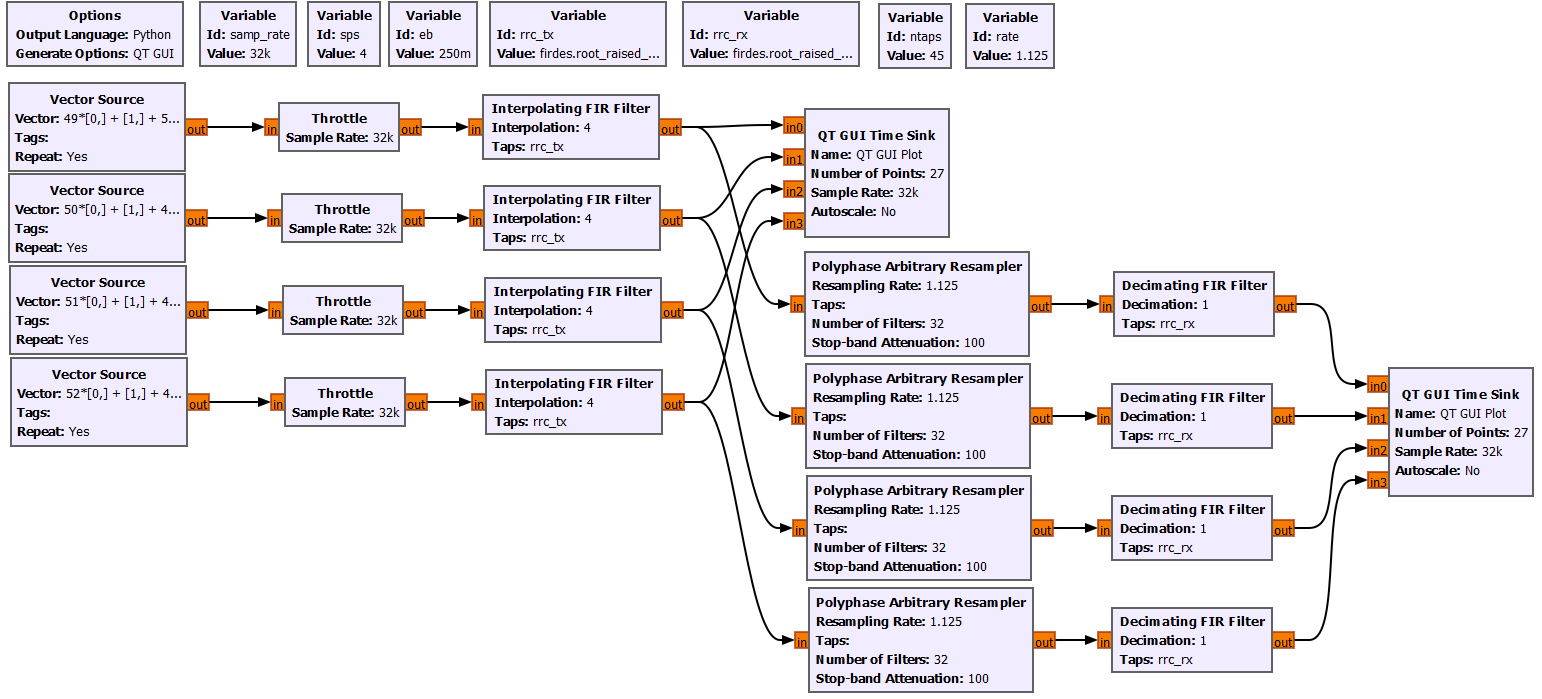
\includegraphics[width=0.8\textwidth]{fig3-3.PNG}
        \caption{Спектры треугольного и пилообразного сигналов}
        \label{fig:fig3-3}
\end{figure}

    Из рис.3.3 видно, что пилообразный сигнал снижается медленнее, чем треугольный.
    
    Теперь посмотрим на прямоугольный сигнал.
\begin{lstlisting}[caption=Сравнение с прямоугольным сигналосм]
    from thinkdsp import SquareSignal

    sawtooth_wave.make_spectrum().plot(color='gray')
    square = SquareSignal(amp=0.5).make_wave(duration=0.5, framerate=40000)
    square.make_spectrum().plot()
    decorate(xlabel='Frequency (Hz)')
\end{lstlisting}

\begin{figure}[H]
        \centering
        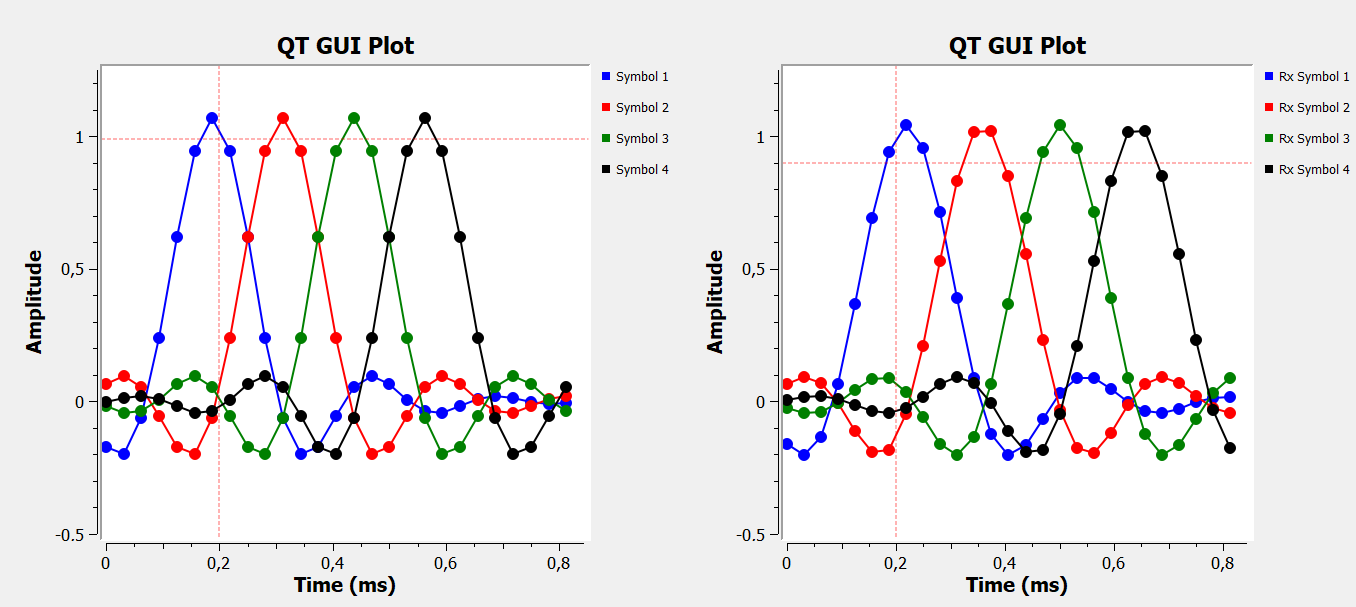
\includegraphics[width=0.8\textwidth]{fig3-4.PNG}
        \caption{Спектры прямоугольного и пилообразного сигналов}
        \label{fig:fig3-4}
\end{figure}    
    
    Из рис.3.4 видно, что пилообразный так же, как и прямоугольный, но у пилообразного есть и чётные, и нечётные гармоники.

\chapter{Упражнение 2.3}
    Создадим прямоугольный сигнал 1100 Гц и вычислим \texttt{wave} с выборками 10000 кадров в секунду. Затем построим спектр этого сигнала.
\begin{lstlisting}[caption=Создание прямоугольного сигнала 1100 Гц]
    from thinkdsp import SquareSignal

    square_wave = SquareSignal(1100).make_wave(duration=0.5, framerate=10000)
    square_wave.make_spectrum().plot()
    decorate(xlabel='Frequency (Hz)')
    square_wave.make_audio()
\end{lstlisting}

\begin{figure}[H]
        \centering
        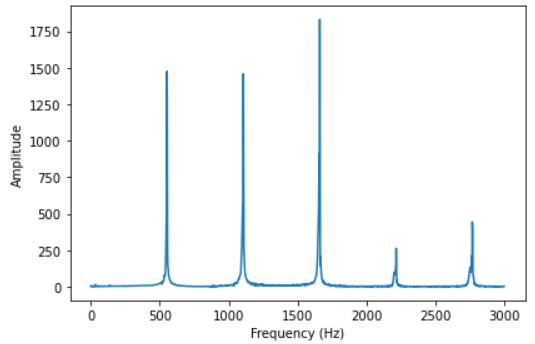
\includegraphics[width=0.8\textwidth]{fig4-1.PNG}
        \caption{Спектр прямоугольного сигнала}
        \label{fig:fig4-1}
\end{figure}    

    Из рис.4.1 видно, что основная гармоника находится на частоте 1100 Гц и первая на - 3300 Гц. Это верно. Но вот вторая гармоника, которая должна быть на 5500 Гц, располагается на 4500 Гц. Третья гармоника также не на месте. Она должна быть на частоте 7700 Гц,но находится на 2400 Гц. И т.д.
    
    Таким образом, мы убедились, что гармоники "завернуты" из-за биения.
    
    Воспроизведём полученный сигнал.В получившимся звуке мы можем услышать гармоники биения. Основной тон, который мы воспринимаем, является гармоникой биения на частоте 200 Гц. 
    
    Для того, чтобы в этом убедиться, сравним с с синусоидой 200 Гц.
\begin{lstlisting}[caption=Создание синусоиды 200 Гц]
    from thinkdsp import SinSignal

    SinSignal(200).make_wave(duration=0.5, framerate=10000).make_audio()
\end{lstlisting} 

\chapter{Упражнение 2.4}  
\section{Треугольный сигнал}
    Проведём следующий эксперемент. Возьмём треугольный сигнал с частотой 440 Гц и \texttt{wave} длительностью 0,01 секунд. Выведем этот сигнал (Рис.5.1).
\begin{lstlisting}[caption=Создание треугольного сигнала 440 Гц]
    triangle_wave = TriangleSignal(440).make_wave(duration=0.01)
    triangle_wave.plot()
    decorate(xlabel='Time (s)')
\end{lstlisting}

\begin{figure}[H]
        \centering
        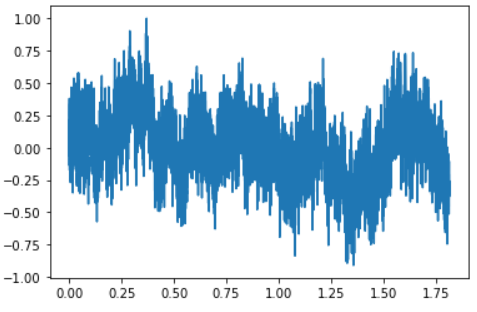
\includegraphics[width=0.8\textwidth]{fig5-1.PNG}
        \caption{Треугольный сигнал}
        \label{fig:fig5-1}
\end{figure}

\section{Объект Spectrum}  
    Создадим объект \texttt{Spectrum} и распечатаем \texttt{Spectrum.hs[0]}.
\begin{lstlisting}[caption=Вывод нулевой компоненты]
    spectrum = triangle_wave.make_spectrum()
    spectrum.hs[0]
\end{lstlisting}   
    
    В результате мы получаем \texttt{(1.0436096431476471e-14+0j)}. Это значение соответствует частотной компоненте: его размах пропорционален амплитуде соответствующей компоненты, а угол в степени числа $e$ – это фаза.

\section{Изменение компоненты}
    Установим \texttt{Spectrum.hs[0] = 100}.
\begin{lstlisting}[caption=Изменение компоненты]
    triangle_wave.plot(color='gray')
    spectrum.hs[0] = 100
    spectrum.make_wave().plot()
    decorate(xlabel='Time (s)')
\end{lstlisting}

\begin{figure}[H]
        \centering
        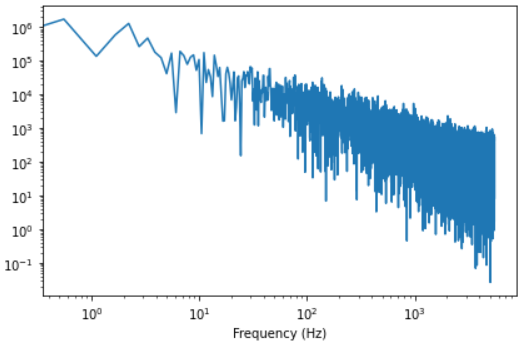
\includegraphics[width=0.8\textwidth]{fig5-2.PNG}
        \caption{Сравнение сигналов}
        \label{fig:fig5-2}
\end{figure}   

    Как можно видеть на рис.5.2 сигнал сместился вверх.

\chapter{Упражнение 2.5}
\section{Создание функции}
    Напишем функцию, принимающую  \texttt{Spectrum} как параметр и изменяющую его делением каждого элемента \texttt{hs} на соответствующую частоту \texttt{fs}.
\begin{lstlisting}[caption=Функция изменения спектра]
def change_spectrum(spectrum):
    spectrum.hs[1:] /= spectrum.fs[1:]
    spectrum.hs[0] = 0
\end{lstlisting} 

\section{Использование функции}
    Проверим эту функцию, используя прямоугольный сигнал. Для этого вычислим \texttt{Spectrum} и распечатаем его (Рис.6.1).
\begin{lstlisting}[caption=Вычисление спектра]
    wave = SquareSignal(freq=440).make_wave(duration=0.5)
    spectrum = wave.make_spectrum()
    spectrum.plot()
    wave.make_audio()
\end{lstlisting}

\begin{figure}[H]
        \centering
        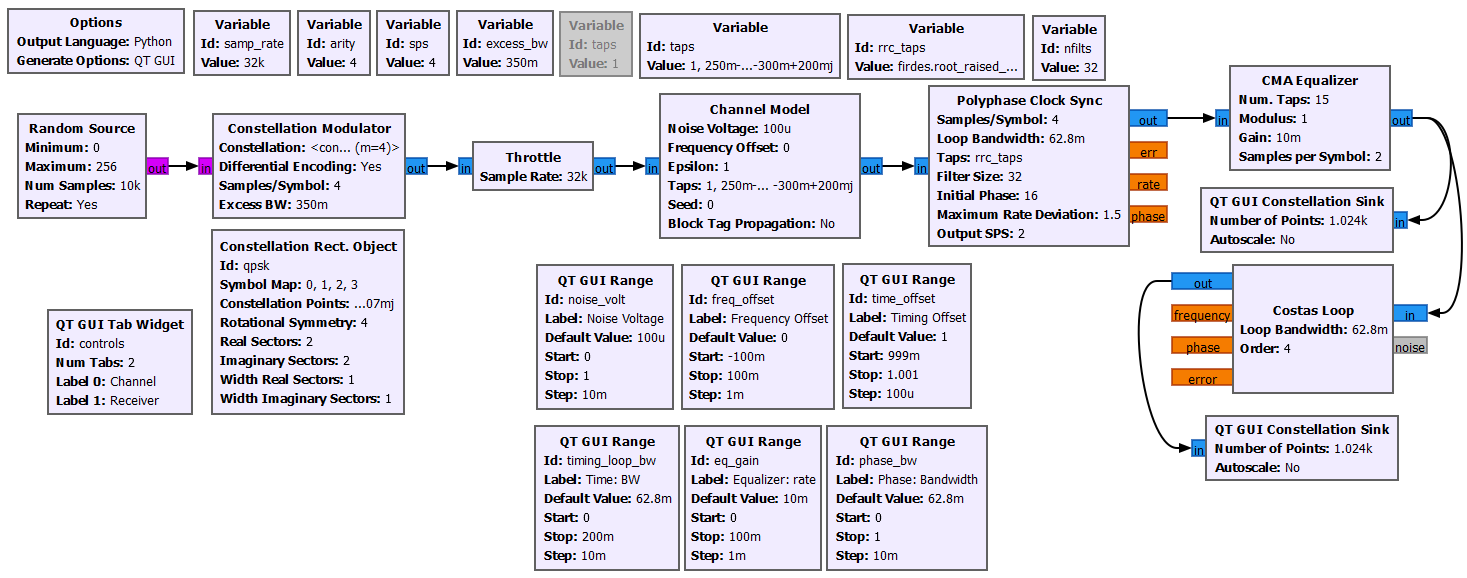
\includegraphics[width=0.8\textwidth]{fig6-1.PNG}
        \caption{Спектр прямоугольного сигнала}
        \label{fig:fig6-1}
\end{figure}   

    Изменим \texttt{Spectrum}, используя нашу функцию, и распечатаем его (Рис.6.2).
\begin{lstlisting}[caption=Вычисление нового спектра]
    spectrum.plot(color='gray')
    change_spectrum(spectrum)
    spectrum.scale(440)
    spectrum.plot()
    decorate(xlabel='Frequency (Hz)')
\end{lstlisting}

\begin{figure}[H]
        \centering
        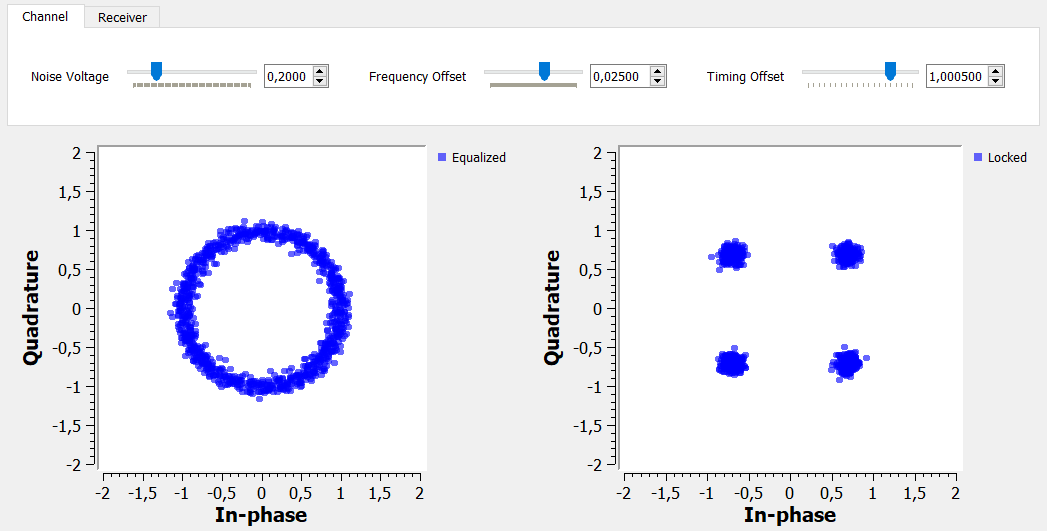
\includegraphics[width=0.8\textwidth]{fig6-2.PNG}
        \caption{Сравнение спектров}
        \label{fig:fig6-2}
\end{figure}     

    Используем \texttt{Spectrum.make\_wave}, чтобы сделать \texttt{wave} из измененного \texttt{Spectrum} и послушаем его.
\begin{lstlisting}[caption=Воспроизведение сигнала]
    spectrum.make_wave().make_audio()
\end{lstlisting}

    Получившийся сигнал стал более приглушённый.
\chapter{Упражнение 2.6} 
    Составим сигнал, который будет состоять из чётных и нечётных гармоник, спадающих пропорционально $1/f^2$. Возьмём пилообразный сигнал, в котором есть все необходимые нам гармоники. Его гармоники спадают пропорционально $1/f$ (Рис.7.1).
\begin{lstlisting}[caption=Создание пилообразного сигнала]
    signal = SawtoothSignal(500)
    wave = signal.make_wave(duration=0.5, framerate=40000)
    spectrum = wave.make_spectrum()
    spectrum.plot()
    decorate(xlabel='Frequency (Hz)')
    wave.make_audio()
\end{lstlisting}

\begin{figure}[H]
        \centering
        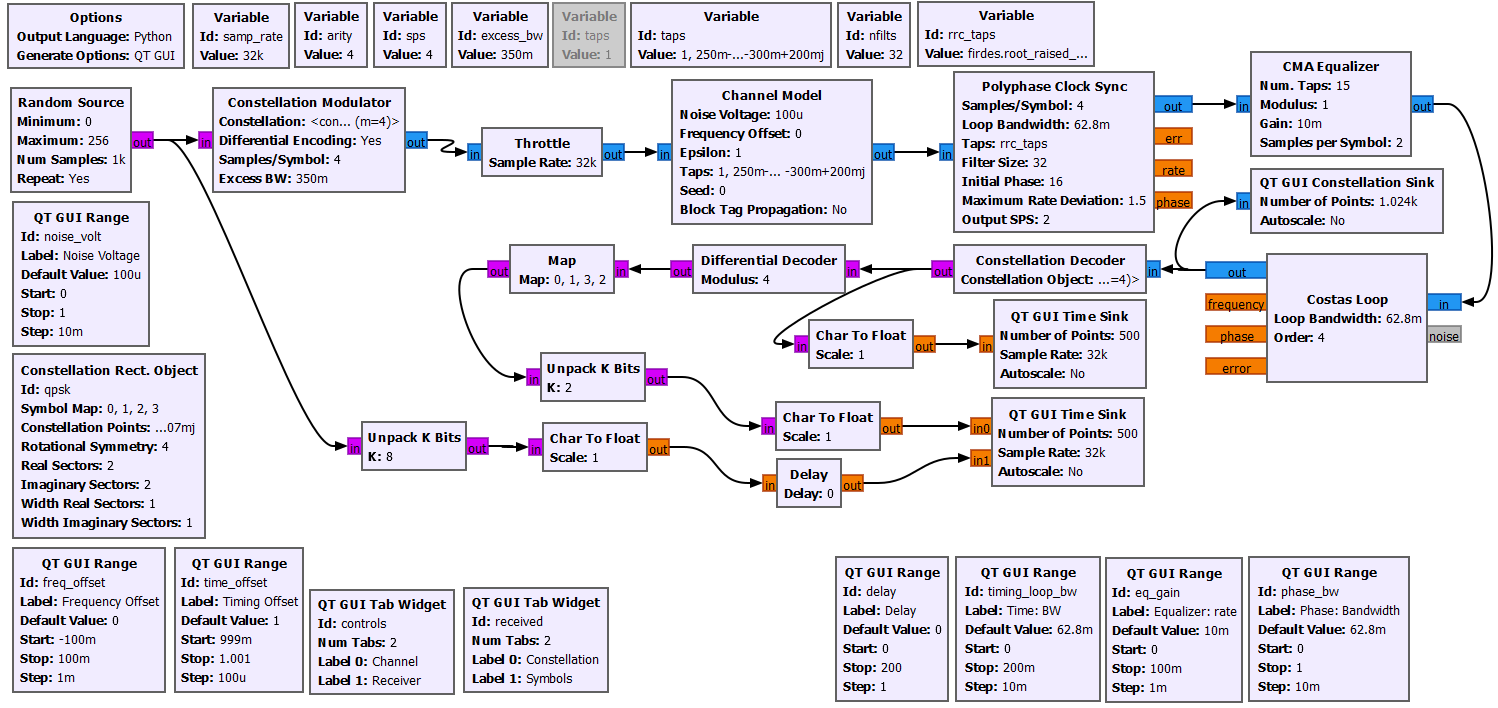
\includegraphics[width=0.8\textwidth]{fig7-1.PNG}
        \caption{Спектр пилообразного сигнала}
        \label{fig:fig7-1}
\end{figure}

    Теперь используем функцию для изменения спектра, написанную в Упражнении 2.6. Если мы применим эту функцию, то мы можем заставить гармоники спадать как $1/f^2$ (Рис.7.2).
\begin{lstlisting}[caption=Применение функции change\_spectrum к сигналу]
    spectrum.plot(color='gray')
    change_spectrum(spectrum)
    spectrum.scale(500)
    spectrum.plot()
    decorate(xlabel='Frequency (Hz)')
\end{lstlisting}

\begin{figure}[H]
        \centering
        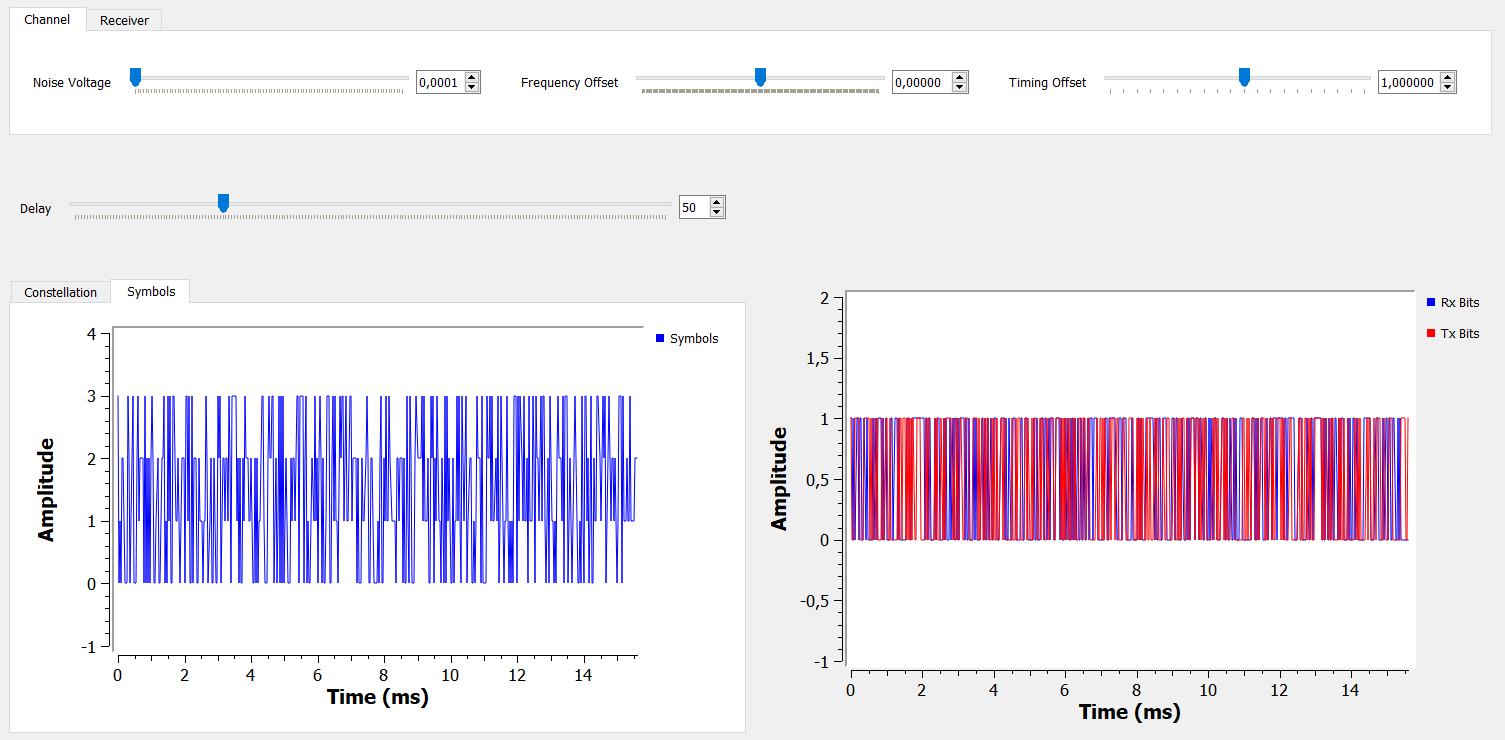
\includegraphics[width=0.8\textwidth]{fig7-2.PNG}
        \caption{Спектр полученного сигнала}
        \label{fig:fig7-2}
\end{figure}

    Полученный сигнал похож на синусоиду (Рис.7.3).
\begin{lstlisting}[caption=Получение сигнала]
    wave = spectrum.make_wave()
    wave.segment(duration=0.01).plot()
    decorate(xlabel='Time (s)')
\end{lstlisting}

\begin{figure}[H]
        \centering
        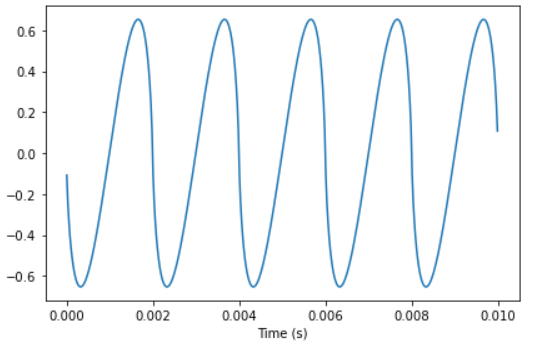
\includegraphics[width=0.8\textwidth]{fig7-3.PNG}
        \caption{Полученный сигнал}
        \label{fig:fig7-3}
\end{figure}

\chapter{Выводы}
    В результате выполнения данный работы мы познакомились некоторыми видами сигналов: треугольным, пилообразным и прямоугольным. Мы получили навыки работы с ними. 
    Также мы изучили биение — эффект, приводящий к наложению различных непрерывных сигналов при их дискретизации.

\begin{thebibliography}{}
    \bibitem{litlink1}  Фильтрация измерительных сигналов / В.С.Гутников.– СПб.:Изд-во Энергоатомиздат, 1990.-192 с.
    \bibitem{litlink2}  Цифровая обработка сигналов / А.С.Сергиенко.– СПб.:Питер, 2003.-603 с.
\end{thebibliography}
\end{document}
    
